\documentclass[../main.tex]{subfiles}
\begin{document}
\begin{center}
\begin{Huge}
RESULTS-Anti-ferromagnetic Trigger
\end{Huge}
\end{center}
%\chapter{Results}\label{ch:A}
This chapter will focus on the effects on the performance of quantum annealing algorithm upon adding the second trigger, namely the anti-ferromagnetic trigger, to the original Hamiltonian. Unlike in the case of the ferromagnetic trigger, for anti-ferromagnetic trigger the strength parameter, g in equation (\ref{eq:b12}) plays a more decisive role than merely controlling the extent by which the minimum gap is enlarged. The anti-ferromagnetic trigger alters the energy spectra, the minimum energy gaps, and the number of anti-crossings between the ground and first excited energy state of the Hamiltonian, depending on the strength with which the trigger is added, as well as on the problem itself. We shall begin by observing the effects of adding the anti-ferromagnetic trigger to the original Hamiltonian, for the three chosen problems. The following sections will then showcase the role that the strength parameter - g plays.

\section*{The chosen problems}
Let us begin by considering the first chosen case, with largest success probability. \\
Figures (\ref{fig:a1}), (\ref{fig:a2}) and (\ref{fig:a3}) show the energy spectra and the instantaneous energy values after adding the anti-ferromagnetic trigger to the first chosen case, with strengths 0.5, 1 and 2 respectively.
\begin{figure}[H]
\centering 
\includegraphics[scale=0.3]{733_s12_A_g0.png}
\caption{The energy spectrum for the first problem, with instantaneous energy values corresponding to three annealing times, with Anti-ferromagnetic trigger, and g=0.5. $\Delta_{min}$ was found to be 0.3070, while $p$=0.9117 for $T_A$=100. }
\label{fig:a1}
\end{figure}
\begin{figure}[H]
\centering 
\includegraphics[scale=0.3]{733_s12_A_g1.png}
\caption{The energy spectrum for the first problem, with instantaneous energy values corresponding to three annealing times, with Anti-ferromagnetic trigger, and g=1. $\Delta_{min}$ was found to be 0.1349, while $p$=0.5747 for $T_A$=100. }
\label{fig:a2}
\end{figure}
\begin{figure}[H]
\centering 
\includegraphics[scale=0.3]{733_s12_A_g2.png}
\caption{The energy spectrum for the first problem, with instantaneous energy values corresponding to three annealing times, with Anti-ferromagnetic trigger, and g=2. $\Delta_{min}$ was found to be 0.0020, while $p$=0.0273 for $T_A$=100. }
\label{fig:a3}
\end{figure}
Table (\ref{tab:a1}) shows a comparison of the success probabilities - p, and minimum energy gaps - $\Delta_{min}$ between the original Hamiltonian and the Hamiltonian after adding the anti-ferromagnetic triggers with different strengths.

\begin{table}[H]
\centering
\renewcommand{\arraystretch}{1.5}
\begin{tabular}{|c|c|c|c|c|}
\hline 
CASE 1 & Original Hamiltonian & Trigger=A, g=0.5 & Trigger=A, g=1 & Trigger=A, g=2 \\ 
\hline 
$\Delta_{min}$ & 0.4407 & 0.3070 & 0.1349 & 0.0020 \\ 
\hline 
p($T_A$=10) & 0.3444 & 0.1446 & 0.0279 & 1.271 $\times 10^{-4}$ \\ 
\hline 
p($T_A$=100) & 0.0044 & 0.9117 & 0.5747 & 0.0273 \\ 
\hline 
p($T_A$=1000) & 0.9999 & 0.9999 & 0.9999 & 0.8761 \\ 
\hline 
s value at $\Delta_{min}$ & 0.459 & 0.367 & 0.282 & 0.254 \\ 
\hline
Number of anti-crossings & 1 & 2 & 1 & 4 \\
\hline
\end{tabular} 
\caption{A comparison of the minimum gaps and the success probabilities for the first chosen case, between the original Hamiltonian and and the Hamiltonian with anti-ferromagnetic trigger (A) of different strengths. The minimum gaps become successively smaller as the strength of the anti-ferromagnetic trigger is increased. The success probabilities are decreased as a result. The value of s corresponding to the position of the minimum gap also becomes smaller.}
\label{tab:a1}
\end{table}
As can be noted from the table above, the minimum energy gap decreases upon adding the ferromagnetic trigger, and this decrease becomes larger as the strength of the trigger is increased. Consequently, the success probabilities (after adding the trigger) are found to be decreasing as well. The value of annealing parameter - s also become smaller with increasing strength of the trigger.
A new feature observed after adding the anti-ferromagnetic trigger is the change in the number of anti-crossings between the ground and the first energy state. For strengths g=0.5 and g=2, the number of energy anti-crossings increase to 2 and 4 respectively, while for g=1 it remains unchanged. Moreover, when the anti-ferromagnetic trigger is added with strength 2, the energy spectrum changes quite drastically in comparison to the original spectrum (\ref{fig:o2}), as can be more clearly seen in the inset of figure (\ref{fig:a3}).\\

Next, let us consider the second chosen problem that had small success probability in absence of any triggers. Figures (\ref{fig:a4}), (\ref{fig:a5}), and (\ref{fig:a6}) show the energy spectrum and the instantaneous energy values corresponding to three annealing times. 


\begin{figure}[H]
\centering 
\includegraphics[scale=0.3]{950_s12_A_g0.png}
\caption{The energy spectrum for the second problem, with instantaneous energy values corresponding to three annealing times, with Anti-ferromagnetic trigger, and g=0.5. $\Delta_{min}$ was found to be 0.0130, while $p$=0.0022 for $T_A$=100. }
\label{fig:a4}
\end{figure}
\begin{figure}[H]
\centering 
\includegraphics[scale=0.3]{950_s12_A_g1.png}
\caption{The energy spectrum for the second problem, with instantaneous energy values corresponding to three annealing times, with Anti-ferromagnetic trigger, and g=1. $\Delta_{min}$ was found to be 0.0019, while $p$=0.0239 for $T_A$=100. }
\label{fig:a5}
\end{figure}
\begin{figure}[H]
\centering 
\includegraphics[scale=0.3]{950_s12_A_g2.png}
\caption{The energy spectrum for the second problem, with instantaneous energy values corresponding to three annealing times, with Anti-ferromagnetic trigger, and g=2. $\Delta_{min}$ was found to be 0.1784, while $p$=0.4468 for $T_A$=100. }
\label{fig:a6}
\end{figure}
For this case, table (\ref{tab:a2}) shows a comparison of the minimum energy gaps, and success probabilities (corresponding to different annealing times) between the original Hamiltonian and the Hamiltonian upon adding the anti-ferromagnetic trigger with different strengths. 

\begin{table}[H]
\centering
\renewcommand{\arraystretch}{1.5}
\begin{tabular}{|c|c|c|c|c|}
\hline 
CASE 2 & Original Hamiltonian & Trigger=A, g=0.5 & Trigger=A, g=1 & Trigger=A, g=2 \\ 
\hline 
$\Delta_{min}$ & 0.0312 & 0.0130 & 0.0019 & 0.1784 \\ 
\hline 
p($T_A$=10) & 2.343 $\times 10^{-4}$ & 0.0567 & 0.0017 & 0.0071\\ 
\hline 
p($T_A$=100) & 0.0146 & 0.0022 & 0.0239 & 0.4468 \\ 
\hline 
p($T_A$=1000) & 0.1362 & 0.0228 & 0.1729 & 0.9999 \\ 
\hline 
s value at $\Delta_{min}$ & 0.665 & 0.644 & 0.601 & 0.263 \\ 
\hline 
Number of anti-crossings & 1 & 1 & 2 & 3 \\
\hline
\end{tabular} 
\caption{A comparison of the minimum gaps and the success probabilities for the second chosen case, between the original Hamiltonian and and the Hamiltonian with anti-ferromagnetic trigger (A) of different strengths. The minimum gap becomes small for g=0.5, and even smaller for g=1, while it becomes even larger than the original minimum energy gap for g=2. The value of s corresponding to the position of the minimum gap becomes smaller with increasing strength of the trigger.}
\label{tab:a2}
\end{table}


The minimum energy gaps decrease with respect to the original energy gaps upon adding the trigger with strengths 0.5, and 1. However, the success probability at $T_A$=10 for anti-ferromagnetic trigger with g=0.5 and g=1 is larger compared to that of the original Hamiltonian, owing to different reasons.\\

Since upon adding the anti-ferromagnetic trigger with strength 0.5, the minimum energy gap becomes smaller, the annealing time of $T_A$=10 is so short that the state of the system transits to the first excited state even before the minimum gap anti-crossing. Upon approaching the minimum gap anti-crossing the system state shifts some of the amplitude back to the ground state, increasing the success probability in this case (figure \ref{fig:a4}). However, for the original Hamiltonian the gap is large enough for an annealing time of 10 for the state to not shift to the first excited state before the minimum energy gap (figure \ref{fig:o3}). The state therefore stays close to the first excited state after passing the anti-crossing.
Furthermore, for annealing times $T_A$=100 and $T_A$=1000, the system state transitions only at the minimum gap anti-crossing and closely follows the second and first excited states respectively. The overlap with the ground state decreases, and therefore the success probability in both these cases also reduces.\\

For the other case - with anti-ferromagnetic trigger with strength 1, the number of energy anti-crossings increases to 2. The first energy anti-crossing is small enough for just $T_A$=10 to shift the system state to the first excited state. Quickly after transitioning to the first excited state, the system state shifts to higher energy levels (figure \ref{fig:a5}). Since the state of the system is a superposition of many energy eigenstates, the present state of system has small, yet finite overlap with the ground state. In the original Hamiltonian, however, the system state shifts to the first excited state at the only energy anti-crossing, and therefore the overlap with the ground state becomes negligible (figure \ref{fig:o3}).\\

By choosing the strength to be 2, the minimum energy gap of this problem becomes larger than the original minimum energy gap, while the number of anti-crossings between the ground and the first excited state increases to 3. The success probability in this case is always larger than the original success probability for all annealing times. For $T_A$=10, the state of the system shifts to the first excited state at first energy anti-crossing, and then quickly shifts to a superposition state with the higher energy states. This results in a larger overlap with the ground state compared to the case of the state closely following the first excited state after reaching the only energy anti-crossing in case of the original problem (\ref{fig:o3}).

For $T_A$=100, the state starts transitioning to the first excited state only as it approaches the second energy anti-crossing. The state does further shift to higher energy levels, but comes back to the first excited state before the third energy anti-crossing. After passing by the third anti-crossing some of the amplitude of the wave function shifts to the ground state again, and therefore the success becomes larger than the original problem. 


Finally, for $T_A$=1000, the annealing time and the minimum energy gap is large enough for the system to always stay close to the ground state, hence the larger success probability.\\

Lastly, figures (\ref{fig:a7}), (\ref{fig:a8}) and (\ref{fig:a9}) show the energy spectra and instantaneous energy values for the third problem, after adding the anti-ferromagnetic trigger with strengths 0.5, 1 and 2 respectively. 


\begin{figure}[H]
\centering 
\includegraphics[scale=0.3]{528_s12_A_g0.png}
\caption{The energy spectrum for the third problem, with instantaneous energy values corresponding to three annealing times, with Anti-ferromagnetic trigger, and g=0.5. $\Delta_{min}$ was found to be 0.0049, while $p$=0.0120 for $T_A$=100. }
\label{fig:a7}
\end{figure}
\begin{figure}[H]
\centering 
\includegraphics[scale=0.3]{528_s12_A_g1.png}
\caption{The energy spectrum for the third problem, with instantaneous energy values corresponding to three annealing times, with Anti-ferromagnetic trigger, and g=1. $\Delta_{min}$ was found to be 0.0562, while $p$=0.1517 for $T_A$=100. }
\label{fig:a8}
\end{figure}
\begin{figure}[H]
\centering 
\includegraphics[scale=0.3]{528_s12_A_g2.png}
\caption{The energy spectrum for the third problem, with instantaneous energy values corresponding to three annealing times, with Anti-ferromagnetic trigger, and g=2. $\Delta_{min}$ was found to be 0.1008, while $p$=0.0480 for $T_A$=100. }
\label{fig:a9}
\end{figure}

Table (\ref{tab:a3}) shows a comparison of the minimum energy gaps, and success probabilities (corresponding to different annealing times) between the original Hamiltonian and the Hamiltonian upon adding the anti-ferromagnetic trigger with different strengths. 

\begin{table}[H]
\centering
\renewcommand{\arraystretch}{1.5}
\begin{tabular}{|c|c|c|c|c|}
\hline 
CASE 3 & Original Hamiltonian & Trigger=A, g=0.5 & Trigger=A, g=1 & Trigger=A, g=2 \\ 
\hline 
$\Delta_{min}$ & 0.1573 & 0.0049 & 0.0562 & 0.1008 \\ 
\hline 
p($T_A$=10) & 0.1577 & 0.0573 & 0.0368 & 4.21 $\times 10^{-5}$\\ 
\hline 
p($T_A$=100) & 0.5199 & 0.0120 & 0.1517 & 0.0480 \\ 
\hline 
p($T_A$=1000) & 0.9992 & 0.0071 & 0.6565 & 0.9313 \\ 
\hline 
s value at $\Delta_{min}$ & 0.514 & 0.454 & 0.418 & 0.256 \\ 
\hline 
Number of anti-crossings & 1 & 1 & 3 & 4 \\
\hline
\end{tabular} 
\caption{A comparison of the minimum gaps and the success probabilities for the third chosen case, between the original Hamiltonian and and the Hamiltonian with anti-ferromagnetic trigger (A) of different strengths. The minimum energy gaps after adding the trigger are smaller than the original minimum gap, for all the values of g. They however become large upon increasing the strength of the anti-ferromagnetic trigger. The value of s corresponding to the position of the minimum gap becomes smaller with increasing strength of the trigger.}
\label{tab:a3}
\end{table}

For this problem, it was observed that adding the anti-ferromagnetic trigger made the minimum energy gaps smaller than the original gap, for all the three values of the strength chosen. The gaps however increased with increasing the strength of the trigger. The original success probabilities, for all annealing times, are therefore larger than the resulting success probabilities upon adding the triggers with different g. Additionally, for all annealing times but $T_A$=10, the success probabilities become larger when the anti-ferromagnetic trigger is added with strength 1 compared to when added with strength 0.5, as the minimum energy gap for the former is larger. For $T_A$=10, and both g=0.5 and g=1 cases, the system state transitions to the first excited state prior to the first energy anti-crossing. This is followed by the state shifting to higher energy levels soon after. Since the energy spectrum becomes more complex (in terms of the number of anti-crossings between the higher energy states and their proximity,) as the strength of the trigger is increased, the system state shifts farther away from the ground state. Consequently, the success probability decreases in the case with g=0.5.

 Although the gap becomes even larger with g=2, the success probability is smaller compared the case with g=1. This can be explained by observing that adding the anti-ferromagnetic trigger with g=2 changes the energy spectrum of the Hamiltonian even more drastically. Not only do the number of anti-crossings between the ground and the first excited state increase to 4, the higher lying energy levels also become more involved and have larger number of anti-crossings. Hence, as annealing times $T_A$=10 and $T_A$=100 are not large enough for the state to stay close to the ground state upon reaching the first energy anti-crossing, the system state settles even farther away from the ground state as compared to the g=1 case. Hence, the success probability for $T_A$=10 and g=2 case is negligible. As the annealing time is increased further to $T_A$=1000, the minimum energy gap becomes large enough to keep the state of the system close to the ground state, and the success probability becomes comparable to the original success probability.
 
 
\section*{g=0.5}
This section will focus on the performance of the quantum annealing algorithm upon adding the anti-ferromagnetic trigger to each of the original Hamiltonian from 12-spin SAT problems, with strength 0.5. For each problem, annealing time was chosen to be 10, 100 and 1000. 

As a measure of quantifying the performance with respect to the original Hamiltonian, a metrics Relative success probability was defined as the ratio of the success probability upon adding the anti-ferromagnetic trigger ($p^A$) to the original success probability ($p^O$). Figures (\ref{fig:a10}), (\ref{fig:a11}) and (\ref{fig:a12}) show the  distribution of the relative success probability for annealing times of 10, 100 and 1000 respectively, with the strength of the trigger Hamiltonian chosen to be 0.5.

\begin{figure}[H]
\centering 
\includegraphics[scale=0.3]{A_T10_g0.png}
\caption{The distribution of relative success probability $\dfrac{p^A}{p^O}$ for g=0.5 and $T_A$=10. 43.9\% of the cases were found to have a higher success probability after adding the trigger.}
\label{fig:a10}
\end{figure}
\begin{figure}[H]
\centering 
\includegraphics[scale=0.3]{A_T100_g0.png}
\caption{The distribution of relative success probability $\dfrac{p^A}{p^O}$ for $T_A$=100. 0.2\% of the cases were found to have a higher success probability after adding the trigger. }
\label{fig:a11}
\end{figure}
\begin{figure}[H]
\centering 
\includegraphics[scale=0.3]{A_T1000_g0.png}
\caption{The distribution of relative success probability $\dfrac{p^A}{p^O}$ for $T_A$=1000. 0.2\% of the cases were found to have a higher success probability after adding the trigger.}
\label{fig:a12}
\end{figure}

For an annealing time $T_A$=10, it was found that 43.9\% of the problems of the set were improved after the anti-ferromagnetic trigger with g=0.5. On increasing the annealing time to 100 and 1000, the percentage of cases with improved success probability dropped to 0.2\% for both the cases. Furthermore, the largest value of the relative success ratio is a little more than 250 for $T_A$=10, while it reduces to 1.995 for $T_A$=100, and to 1.585 for $T_A$=1000. In order to understand the reasons for this decrease in the performance on increasing the annealing time, the minimum energy gaps of all the problems were calculated after adding the trigger. Figure (\ref{fig:a13}) shows a plot of the minimum energy gaps after adding the anti-ferromagnetic trigger ($\Delta_{min}^A$) with the original minimum energy gaps ($\Delta_{min}^O$).
\begin{figure}[H]
\centering 
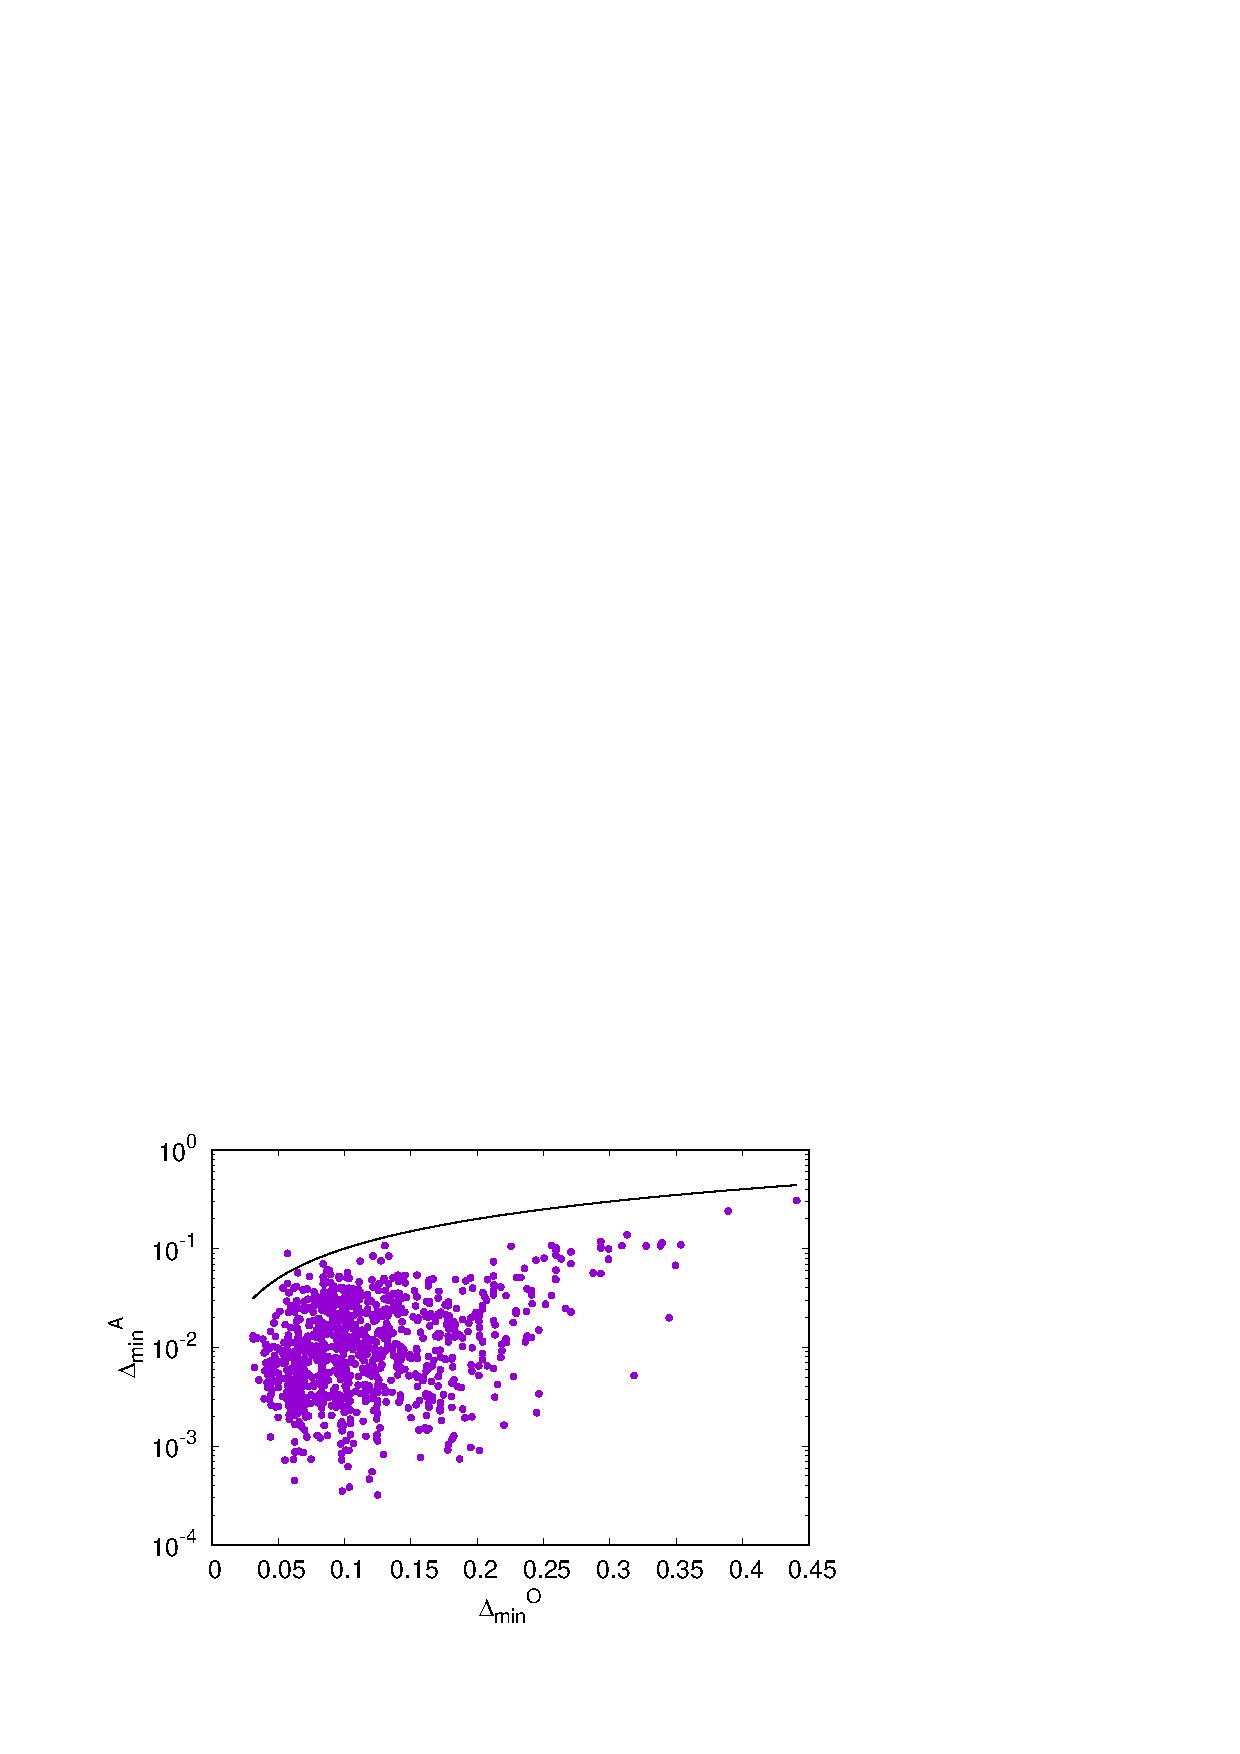
\includegraphics[scale=0.24]{MinGap_A_g0.png}
\caption{A plot of the minimum energy gaps after adding the anti-ferromagnetic trigger with g=0.5 ($\Delta_{min}^A$), with the original minimum energy gaps ($\Delta_{min}^O$). For 99.9\% of the minimum energy gap was found to have decreased after adding the trigger.}
\label{fig:a13}
\end{figure}
As is clear from figure (\ref{fig:a13}), for 99.9\% of the cases, the minimum energy gaps reduce after adding the anti-ferromagnetic trigger with strength 0.5. Additionally, it was found that 92.3\% of all the cases still had a single anti-crossing between the ground and the first excited state, while for the other 7.7\% of the cases, it increased to 2.

For shorter annealing times, like $T_A$=10, the success probability can benefit because of two reasons. As seen in the second chosen problem in the previous section, for small minimum energy gaps, and smaller annealing times, the state of the system can shift to the first excited state prior to the minimum gap anti-crossing. The overlap with the ground state can then increase because of the following non-adiabatic processes:
\begin{itemize}
\item If there are no higher energy states close to the state of the system, the wave function of the state can transfer some amplitude back to the ground state, at one of the anti-crossings.
\item If the higher energy states come close to the system state, before it approaches the energy anti-crossing, the system state can further transit to a superposition state of the higher energy levels. This might increase the overlap of the state with the ground state compared to the case where the state closely follows the first excited state after crossing the energy anti-crossing.
\end{itemize}

Thus, when the annealing time is increased to 100 or 1000, the state of the system stays close to the ground state till it reaches the energy anti-crossing, and transitions to the first excited state afterwards. This explains the drop in the percentage of improved cases upon increasing the annealing time and adding the anti-ferromagnetic trigger. \\

To get an estimate of the difficulty of the affected problems, figure (\ref{fig:a14}) shows the scatter plot of the success probabilities after adding the trigger with the original success probabilities, for the three annealing times. It should be noted that the 43.9\% of the problems improved upon by adding anti-ferromagnetic trigger for $T_A$=10, are the ones that had relatively smaller original success probabilities (harder problems with smaller minimum energy gaps). Adding the anti-ferromagnetic trigger reduces the minimum energy gap, thereby increasing the success probability by either of the two mechanisms listed above.

\begin{figure}[H]
\centering 
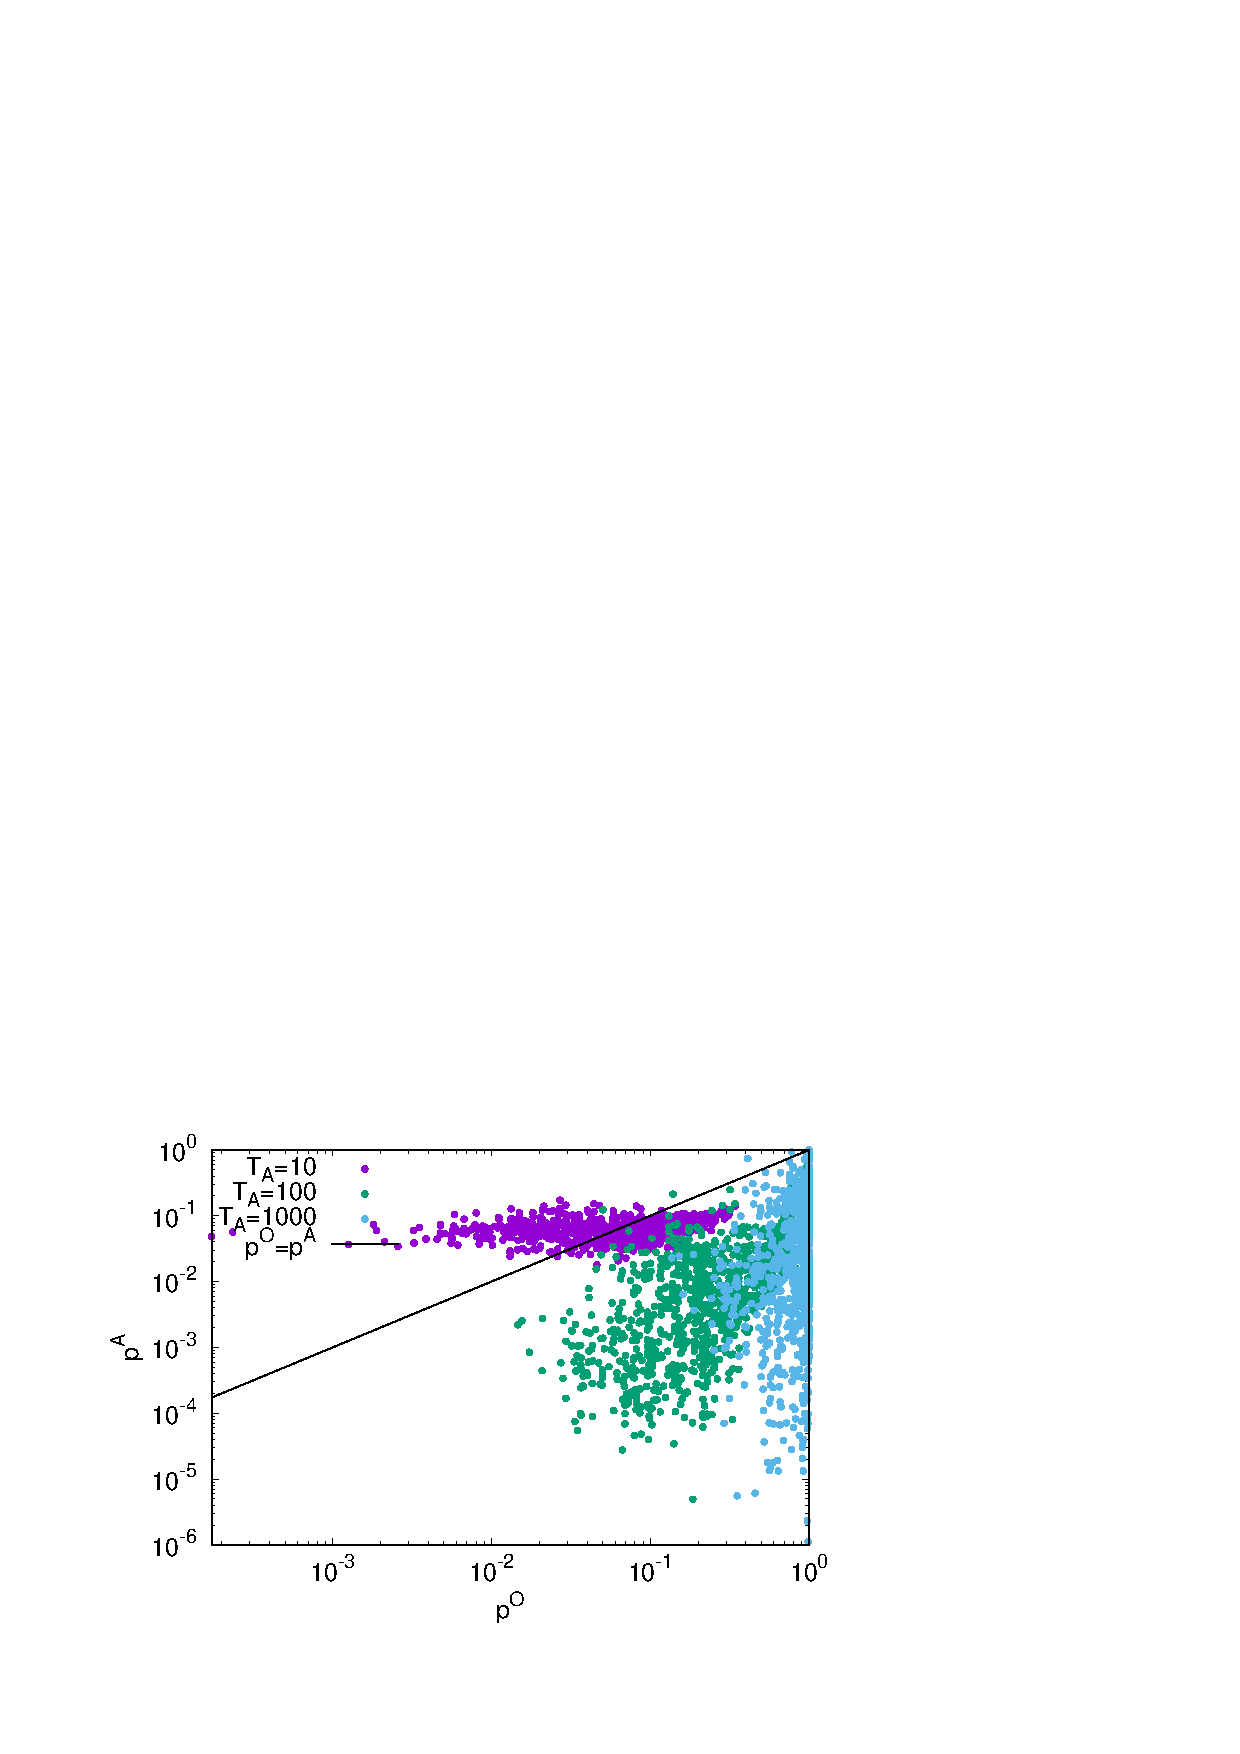
\includegraphics[scale=0.3]{ProbScat_g0.png}
\caption{A plot of the success probabilities after adding the anti-ferromagnetic trigger with g=0.5 ($p^A$), with the original success probabilities($p^O$) for annealing time 10, 100 and 1000.}
\label{fig:a14}
\end{figure}

\begin{figure}[H]
\centering 
\includegraphics[scale=0.3]{Mingap_709_g0_A.png}
\caption{Considered here is the case with increased success probability in spite of a decrease in the minimum energy gap. The energy gap between the two lowest energy levels is compared for this case with that in the original case. The inset shows a comparison with some other problems after adding the trigger. The key difference for the considered case is that the slope of the curve is not symmetric about the point of minimum gap, unlike all other cases. }
\label{fig:a15}
\end{figure}
 
It should also be noted that for $T_A$=100 and $T_A$=1000, the original success probabilities are already quite high, giving way to another reason for the decrease in the relative success probability with increasing annealing time. \\

For both $T_A$=100 and $T_A$=1000 the two problems that had a higher success probability after adding the anti-ferromagnetic trigger, were indeed the same. One of these problem happened to be the only problem that had a larger minimum energy gap upon adding the anti-ferromagnetic trigger, and hence the increase in the success probability. \\
For the other problem, figure (\ref{fig:a15}) shows the energy gap between the ground energy level and the first excited state of the the Hamiltonian (as a function of the annealing parameter), before and after adding the anti-ferromagnetic trigger. The inset of the figure also shows the energy gaps for some other problems after adding the trigger. As can be observed in the figure, the shape of the curve for the case with larger success probability (in spite of the decrease in the minimum energy gap) is different from both the original Hamiltonian and the other problems. The slope in this case, unlike the other cases, is not symmetric about the minimum gap value. While comparing the success probabilities across different problems (and assuming $p=1-e^{-\dfrac{-T {\Delta}^2}{c}}$), the slope (c) for  each problem was supposed to have a similar structure and only changes in the minimum gaps were accounted for. Since this assumption breaks down for this case, the success probability deviates from the expected value.\\

Finally, for checking if the dynamics during the evolution of the state under the action of the anti-ferromagnetic trigger is adiabatic, equation (\ref{eq:lz3}) should be verified, as was done in the last chapter. We plotted the success probability against the minimum energy gaps for all the problems of the set, before and after adding the ferromagnetic trigger, for all the three annealing times. The resulting plot is shown in figure (\ref{fig:a17}).

\begin{figure}[H]
\centering 
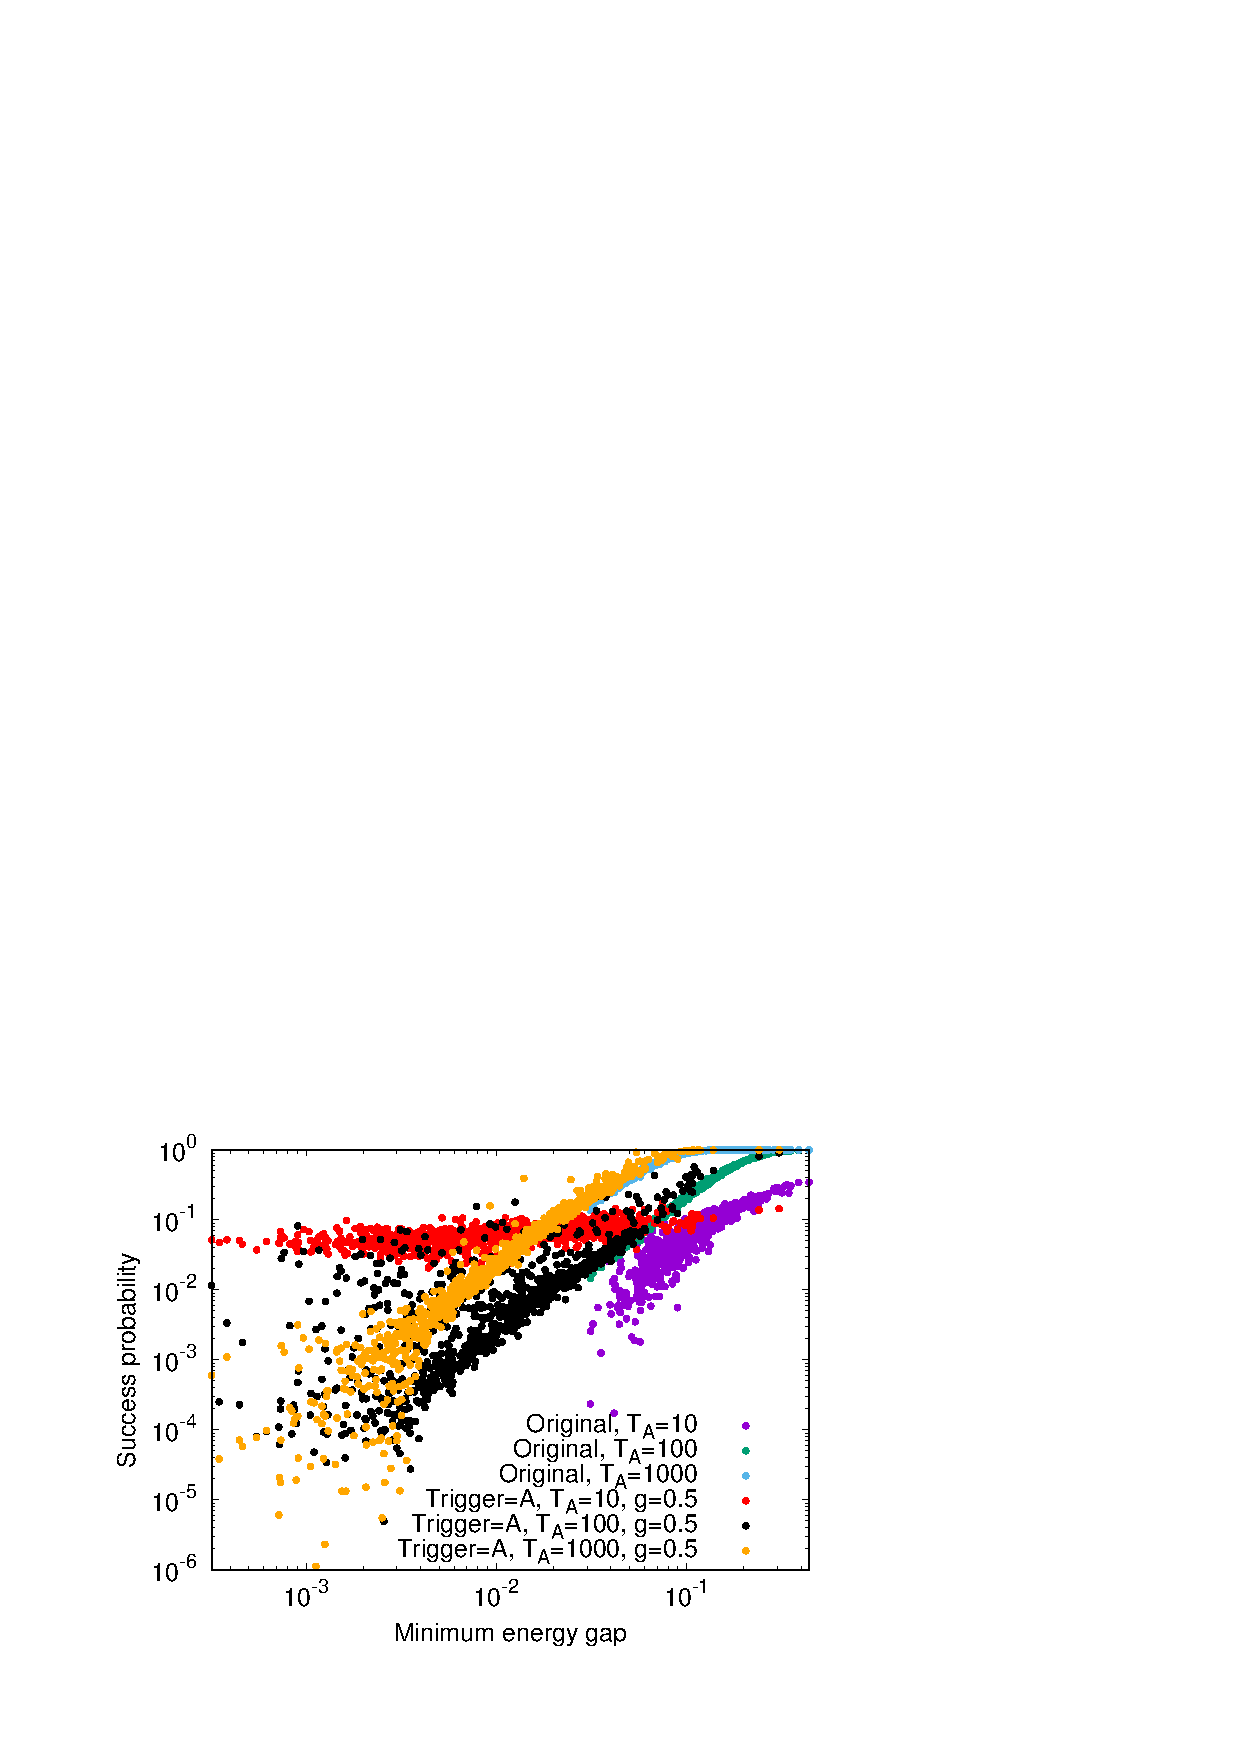
\includegraphics[scale=0.3]{SuccVsGap_OA_g0.png}
\caption{Success probability versus minimum energy plot for all the problems belonging to the set of 12-spin SAT problems, for annealing times 10, 100 an 1000, in the absence and presence of ferromagnetic trigger.}
\label{fig:a17}
\end{figure}


It can be noted from figure (\ref{fig:a17}) that the original success probabilities mostly follow the exponential dependence on minimum energy gaps, although the scattering for $T_A$=10 is comparatively large. As the annealing time is increased, the curve becomes more defined. However, upon adding the trigger, the scattering becomes even larger, so that the points corresponding to $T_A$=10 appear rather flat. Also, for smaller gaps, these points have a higher success probability than the points corresponding to $T_A$=100, due to non-adiabatic evolution. Although in this case too the curves become successively more defined by increasing the annealing time, the general effect of adding the trigger with strength g=0.5 is to shift the data points leftwards by reducing the minimum energy gaps, and thus limiting the performance.



\section*{g=1}
In this section, the same analysis will be shown as in the last section but with the value of the strength parameter set to 1. We begin by showing the distribution of the relative success probability after adding the anti-ferromagnetic trigger with g=1, for annealing times 10, 100 and 1000, in figures (\ref{fig:a18}), (\ref{fig:a19}) and (\ref{fig:a20}) respectively.

\begin{figure}[H]
\centering 
\includegraphics[scale=0.3]{A_T10_g1.png}
\caption{The distribution of relative success probability $\dfrac{p^A}{p^O}$for $T_A$=10. 37.7\% of the cases were found to have a higher success probability after adding the trigger.}
\label{fig:a18}
\end{figure}
\begin{figure}[H]
\centering 
\includegraphics[scale=0.3]{A_T100_g1.png}
\caption{The distribution of relative success probability $\dfrac{p^A}{p^O}$for $T_A$=100. 21.5\% of the cases were found to have a higher success probability after adding the trigger. }
\label{fig:a19}
\end{figure}
\begin{figure}[H]
\centering 
\includegraphics[scale=0.3]{A_T1000_g1.png}
\caption{The distribution of relative success probability $\dfrac{p^A}{p^O}$for $T_A$=1000. 20\% of the cases were found to have a higher success probability after adding the trigger.}
\label{fig:a20}
\end{figure}

37.7\% of the cases had an improved success probability after adding the anti-ferromagnetic trigger for $T_A$=10. This percentage reduced to 21.5\% and 20\% respectively upon increasing the annealing time to 100 and 1000 respectively. Moreover, as the annealing time was increased, the largest value of the relative success probability dropped from 501 at $T_A$=10, to 15.85 at $T_A$=100, to 6.31 at $T_A$=1000. Again, for obtaining more insights about the effects of adding the anti-ferromagnetic trigger with g=1, the minimum energy gaps were computed for all the problems of the set after adding the trigger. Figure (\ref{fig:a21}) shows the resulting scatter plot between the original minimum energy gaps and the gaps after adding the trigger.

\begin{figure}[H]
\centering 
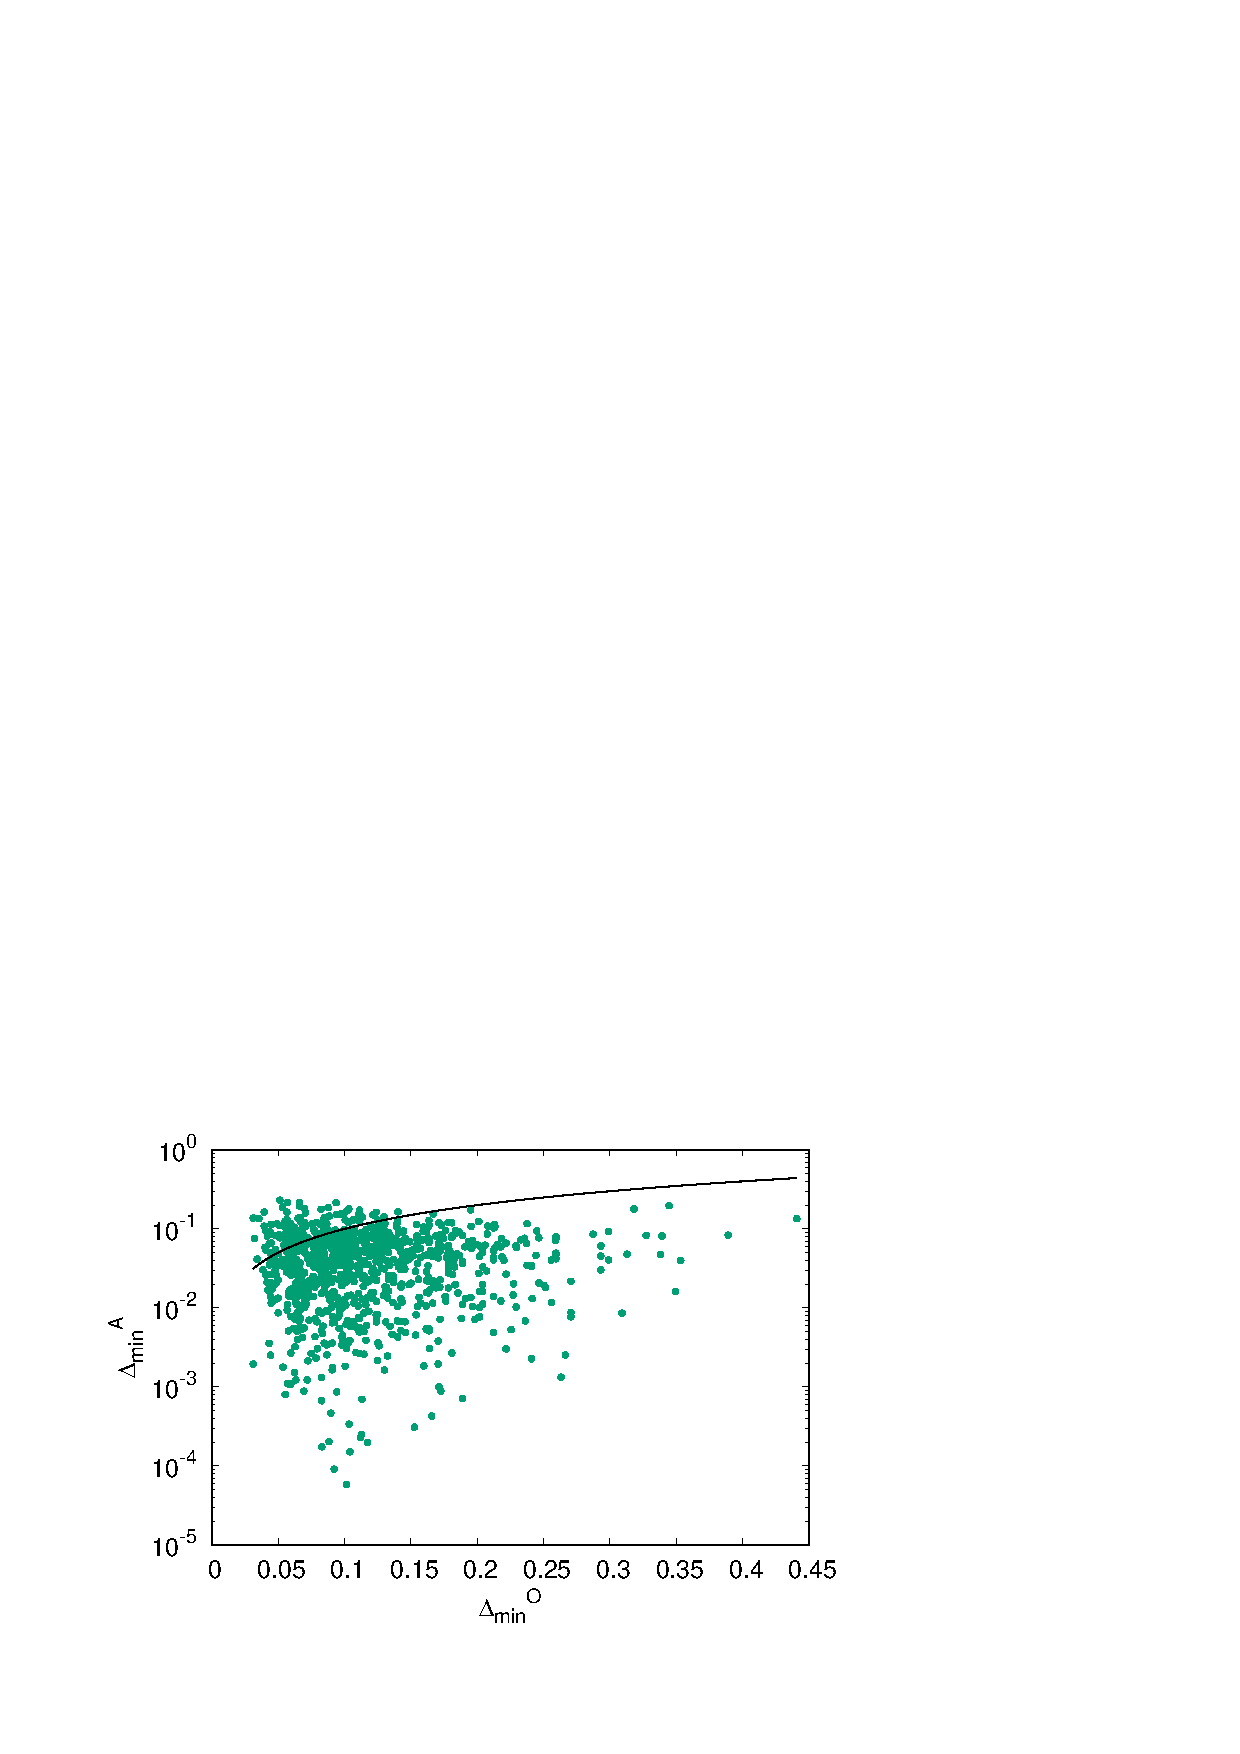
\includegraphics[scale=0.24]{MinGap_A_g1.png}
\caption{A plot of the minimum energy gaps after adding the anti-ferromagnetic trigger with g=1 ($\Delta_{min}^A$), with the original minimum energy gaps ($\Delta_{min}^O$). For 87.9\% of the minimum energy gap was found to have decreased after adding the trigger.}
\label{fig:a21}
\end{figure}
In this case 87.9\% of the cases were found to have smaller minimum energy gaps upon the addition of the trigger. Thus, a decrease in the success probability for most of the cases compared to the original seems to be plausible.

Furthermore, for most of the cases the number of  energy anti-crossings between the ground state and the first excited state increased to 2, while in one case it was noted to be 4. Table (\ref{tab:a4}) shows the percentage of cases for different number of anti-crossings.

\begin{table}[H]
\centering
\renewcommand{\arraystretch}{1.5}
\begin{tabular}{|c|c|}
\hline 
Number of anti-crossings & Number of cases (\%) \\ 
\hline 
1 & 20.2 \\ 
\hline 
2 & 70.5 \\ 
\hline 
3 & 9.2 \\ 
\hline 
4 & 0.1 \\ 
\hline 
\end{tabular} 
\caption{Number of cases with different number of anti-crossings after adding the anti-ferromagnetic trigger.}
\label{tab:a4}

\end{table}
For obtaining an estimate for the difficulty of the problems which have a relative success ratio greater than one, a scatter plot of the original success probability and that after adding the anti-ferromagnetic trigger has been shown in figure (\ref{fig:a22}).


\begin{figure}[H]
\centering 
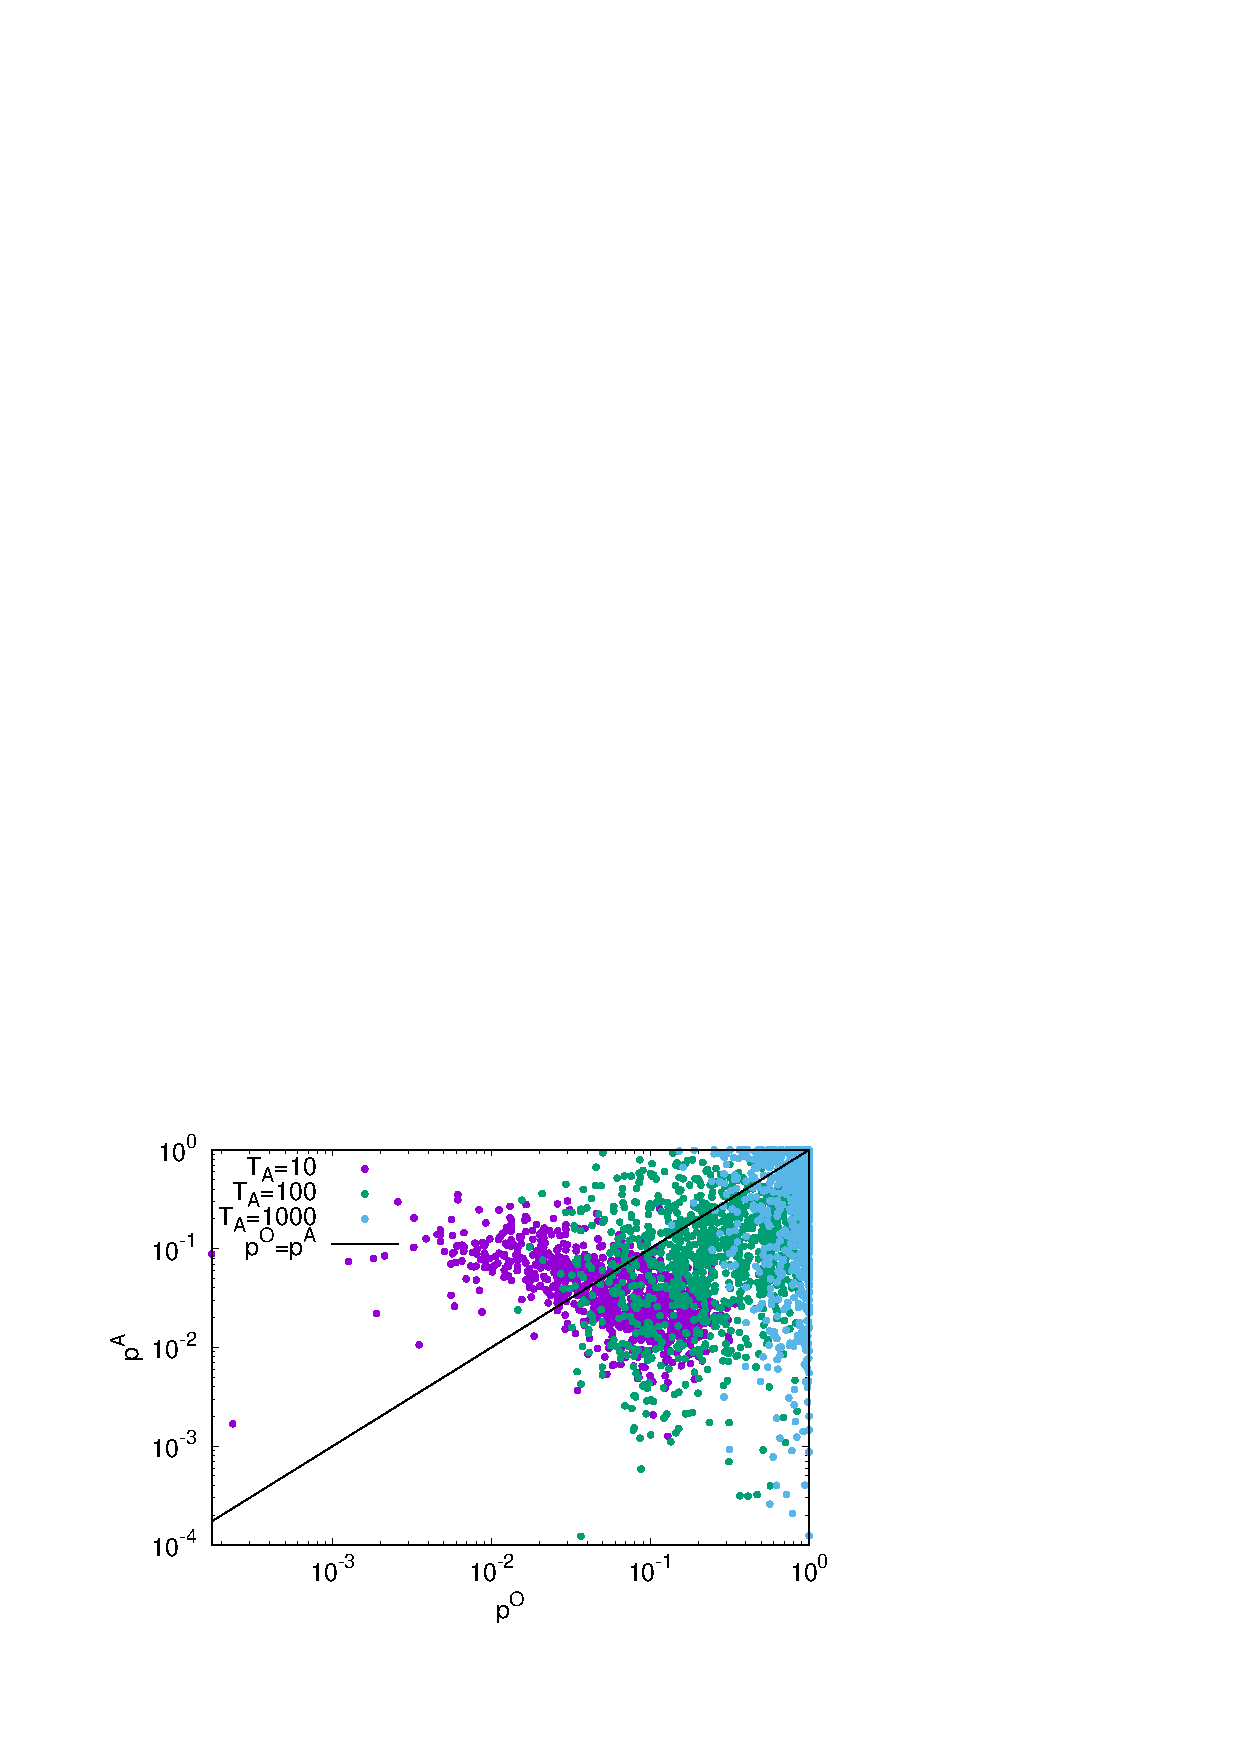
\includegraphics[scale=0.3]{ProbScat_g1.png}
\caption{A plot of the success probabilities after adding the anti-ferromagnetic trigger with g=1 ($p^A$), with the original success probabilities($p^O$) for annealing time 10, 100 and 1000.}
\label{fig:a22}
\end{figure}

Again, it can be noted that the 37.7\% of the problems that have a higher success probability after adding the anti-ferromagnetic trigger are limited to the cases with smaller original success probability (smaller gaps). Since adding the trigger reduces the minimum energy gap in most of the cases, the cases with smaller $p^O$ benefit from a non-adiabatic evolution (shorter annealing time).\\

For understanding the role that the annealing time plays in improving the success probability, scatter plots of original and modified minimum gaps (upon adding the trigger) were plotted for the cases with relative success probability higher than 1, for the three annealing times. These plots have been shown in figure .
(\ref{fig:a23}), (\ref{fig:a26}) and (\ref{fig:a27}).\\

Out of the 37.7\% of the cases with higher success probability after adding the trigger for $T_A$=10, 27.9\% of the cases were found to have smaller minimum gaps as a result of adding the trigger. These cases can therefore be expected to have a non-adiabatic evolution at $T_A$=10, explaining the observed trend. On the other hand, for the rest 9.8\% of the cases the minimum gaps were increased. It was noted that except for 2 cases with larger minimum gaps that were improved for $T_A$=10, were also improved for $T_A$=100 and $T_A$=1000. This suggests that for these cases adding the anti-ferromagnetic trigger increased the minimum energy gap, making the evolution more adiabatic even for $T_A$=10. 

Additionally, for the two cases with enlarged minimum gap and higher success probability for $T_A$=10 but not for $T_A$=100, the energy spectra and instantaneous energies were studied. Same mechanics were found to be governing the trend, therefore the energy spectra for one of the problems is shown here. Figures (\ref{fig:a24}) and (\ref{fig:a25}) show the energy spectrum and the instantaneous energies before and after adding the trigger.

\begin{figure}[H]
\centering 
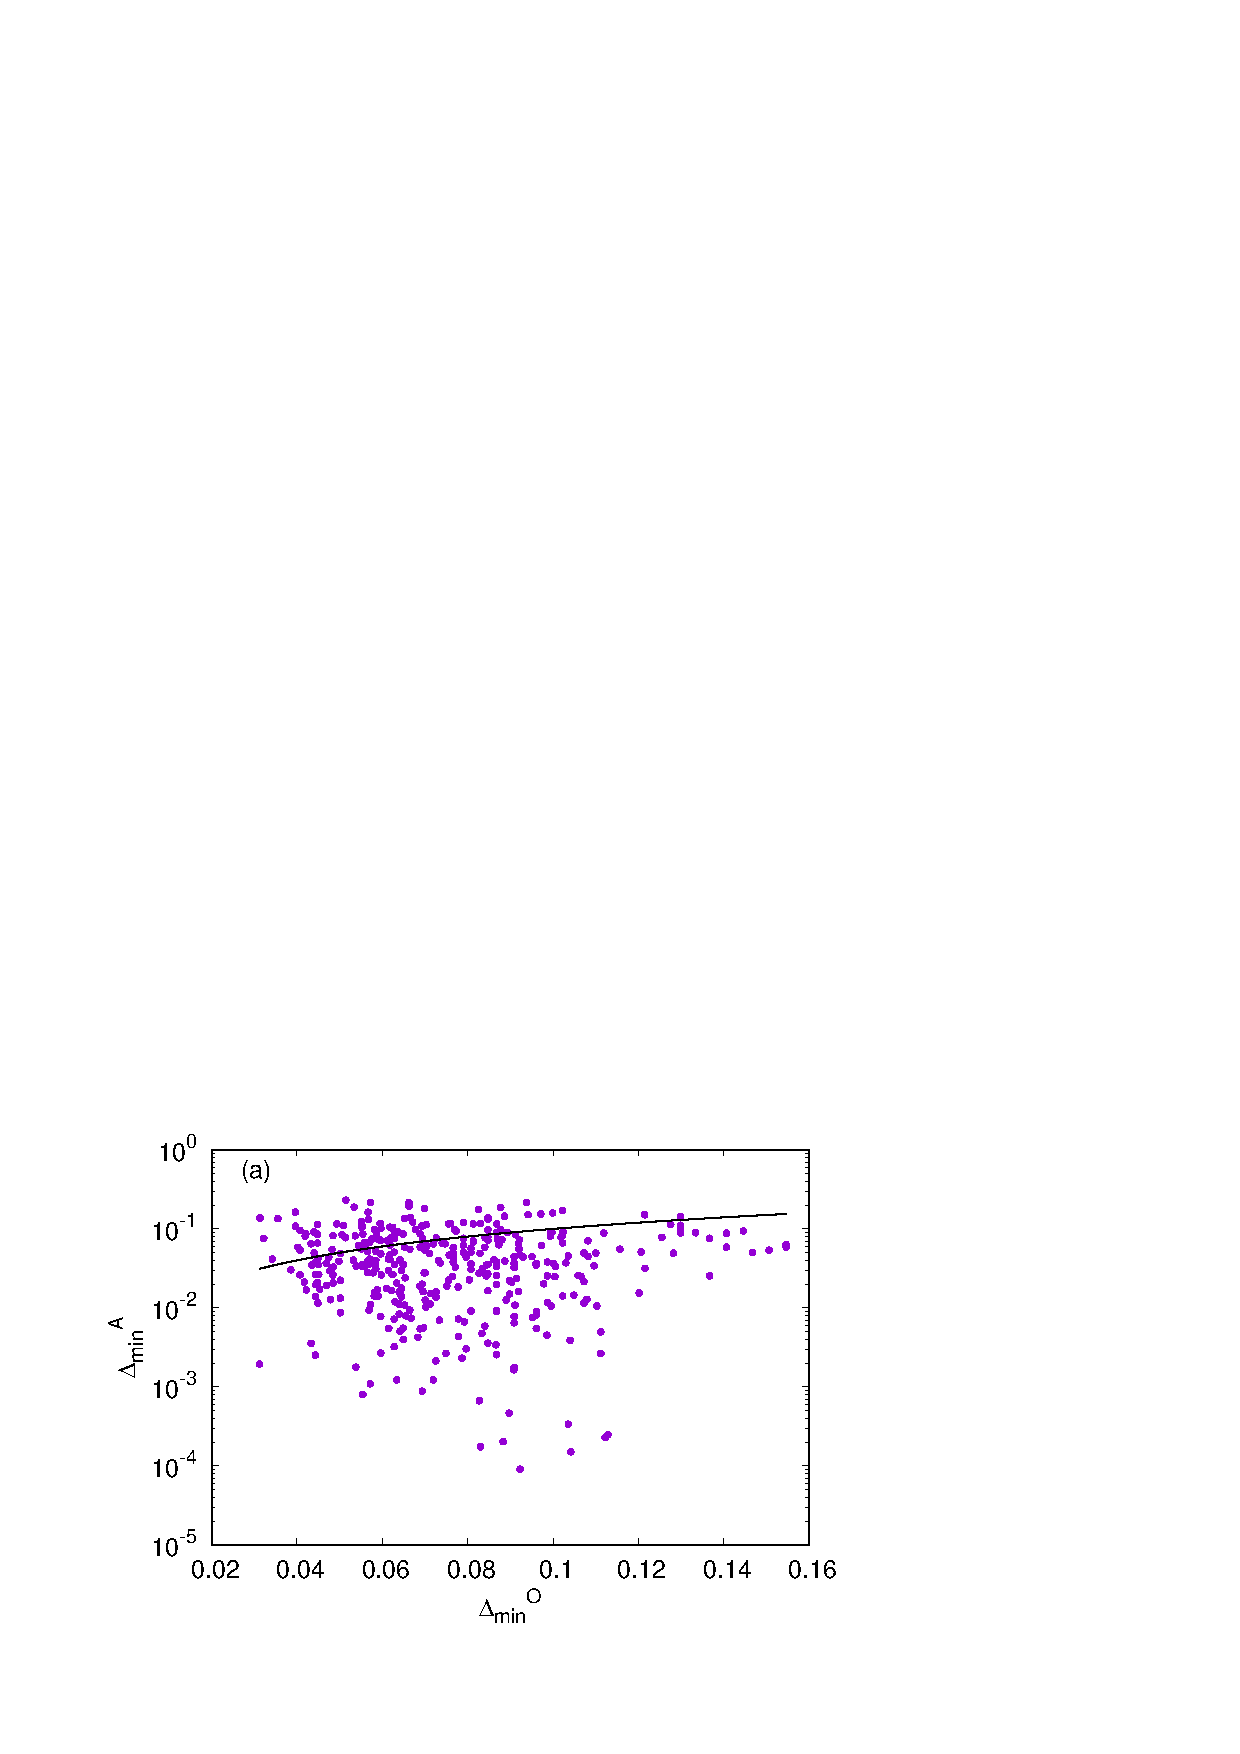
\includegraphics[scale=0.26]{selected_T10_g1.png}
\caption{A plot of the success probabilities after adding the anti-ferromagnetic trigger with g=1 ($p^A$), with the original success probabilities($p^O$) for annealing time 10, 100 and 1000.}
\label{fig:a23}
\end{figure}

\begin{figure}[H]
\centering 
\includegraphics[scale=0.3]{705_O_T.png}
\caption{A plot of the success probabilities after adding the anti-ferromagnetic trigger with g=1 ($p^A$), with the original success probabilities($p^O$) for annealing time 10, 100 and 1000.}
\label{fig:a24}
\end{figure}
\begin{figure}[H]
\centering 
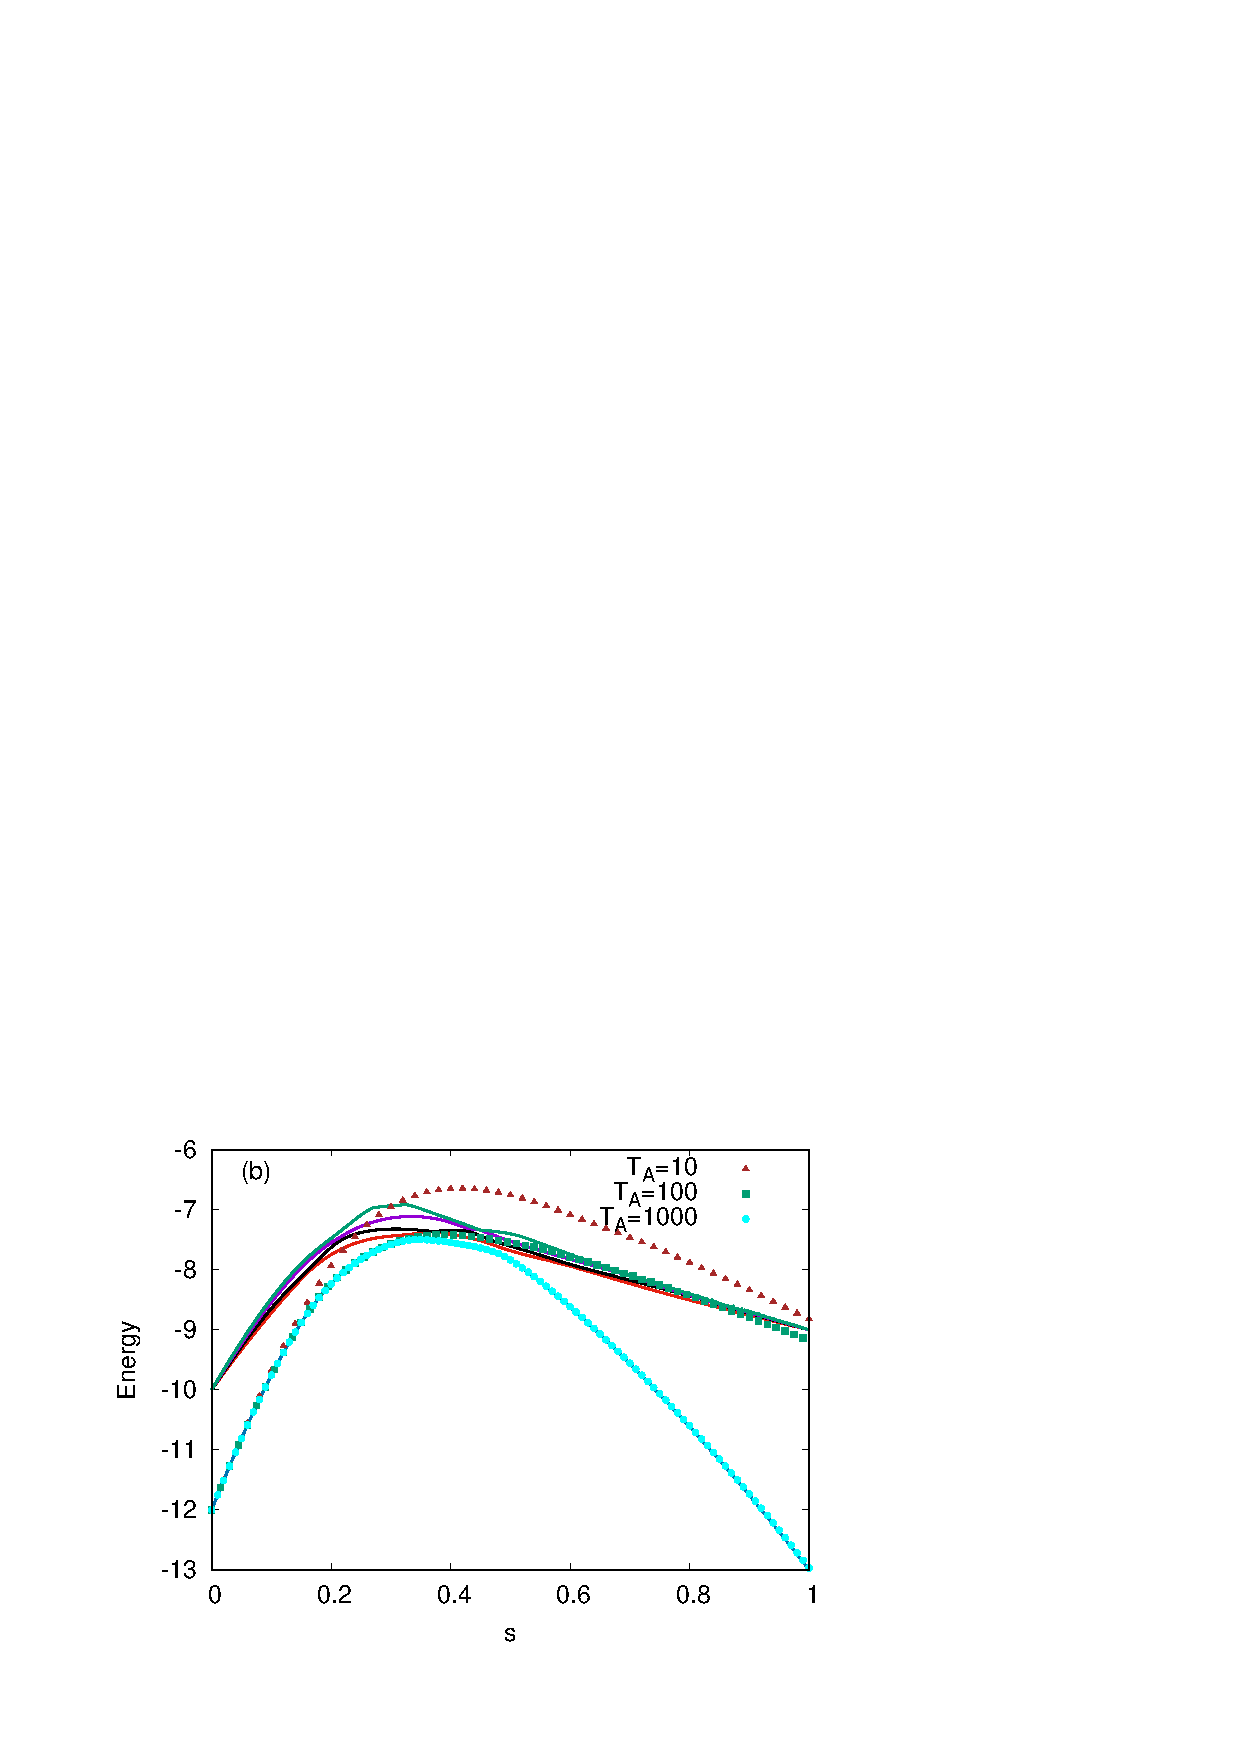
\includegraphics[scale=0.3]{705_A_T_g1.png}
\caption{A plot of the success probabilities after adding the anti-ferromagnetic trigger with g=1 ($p^A$), with the original success probabilities($p^O$) for annealing time 10, 100 and 1000.}
\label{fig:a25}
\end{figure}
Although adding the trigger enlarges the minimum gap in these cases, the spectrum of the problem is changed in a way that the state has more chances of going to higher energy levels. For $T_A$=10 the system transitions to higher energy levels even before the first energy anti-crossing, and coincidentally ends in a state with larger overlap with the ground state than in the original case where it closely follows the first excited state after the anti-crossing. For $T_A$=100, and in the presence of the trigger, the state shifts to the higher excited state at the second energy anti-crossing, but this time the overlap of the final state with the ground state is smaller than that in the case of the original Hamiltonian. Finally, an annealing time of $T_A$=1000 becomes long enough for the evolution to become adiabatic, and since the minimum energy gap is increased after adding the trigger, the success probability in the presence of the trigger becomes larger.\\

Next, from figures (\ref{fig:a26}) and (\ref{fig:a27}) it can be noted that the majority of the problems improved by adding anti-ferromagnetic trigger, and choosing the annealing time to be $T_A$=10 or $T_A$=1000 correspond to the cases where the minimum energy gaps became larger upon adding the trigger. 11.7\% of the   21.5\% of the cases improved after adding the trigger for $T_A$=100, and 12.1\% of the 20\% of those for $T_A$=1000 had larger minimum gaps after including the trigger.
\begin{figure}[H]
\centering 
\includegraphics[scale=0.43]{selected_T100_g1.png}
\caption{A plot of the success probabilities after adding the anti-ferromagnetic trigger with g=1 ($p^A$), with the original success probabilities($p^O$) for annealing time 10, 100 and 1000.}
\label{fig:a26}
\end{figure}
\begin{figure}[H]
\centering 
\includegraphics[scale=0.43]{selected_T1000_g1.png}
\caption{A plot of the success probabilities after adding the anti-ferromagnetic trigger with g=1 ($p^A$), with the original success probabilities($p^O$) for annealing time 10, 100 and 1000.}
\label{fig:a27}
\end{figure}
Some of the outliers of from the above two plots were selected and their dynamics was studied. Firstly, it should be noted that the cases a-e are the ones that appear in both the figures. Out of them, for cases b, c and d there are exactly two anti-crossings where the energy gap is relatively small and comparable to each other. Figures (\ref{fig:a28}) and (\ref{fig:a29}) show the energy spectrum and the instantaneous energies for case c, in the absence and presence of the trigger, respectively.

\begin{figure}[H]
\centering 
\includegraphics[scale=0.3]{441_O_T100_1000.png}
\caption{A plot of the success probabilities after adding the anti-ferromagnetic trigger with g=1 ($p^A$), with the original success probabilities($p^O$) for annealing time 10, 100 and 1000.}
\label{fig:a28}
\end{figure}
\begin{figure}[H]
\centering 
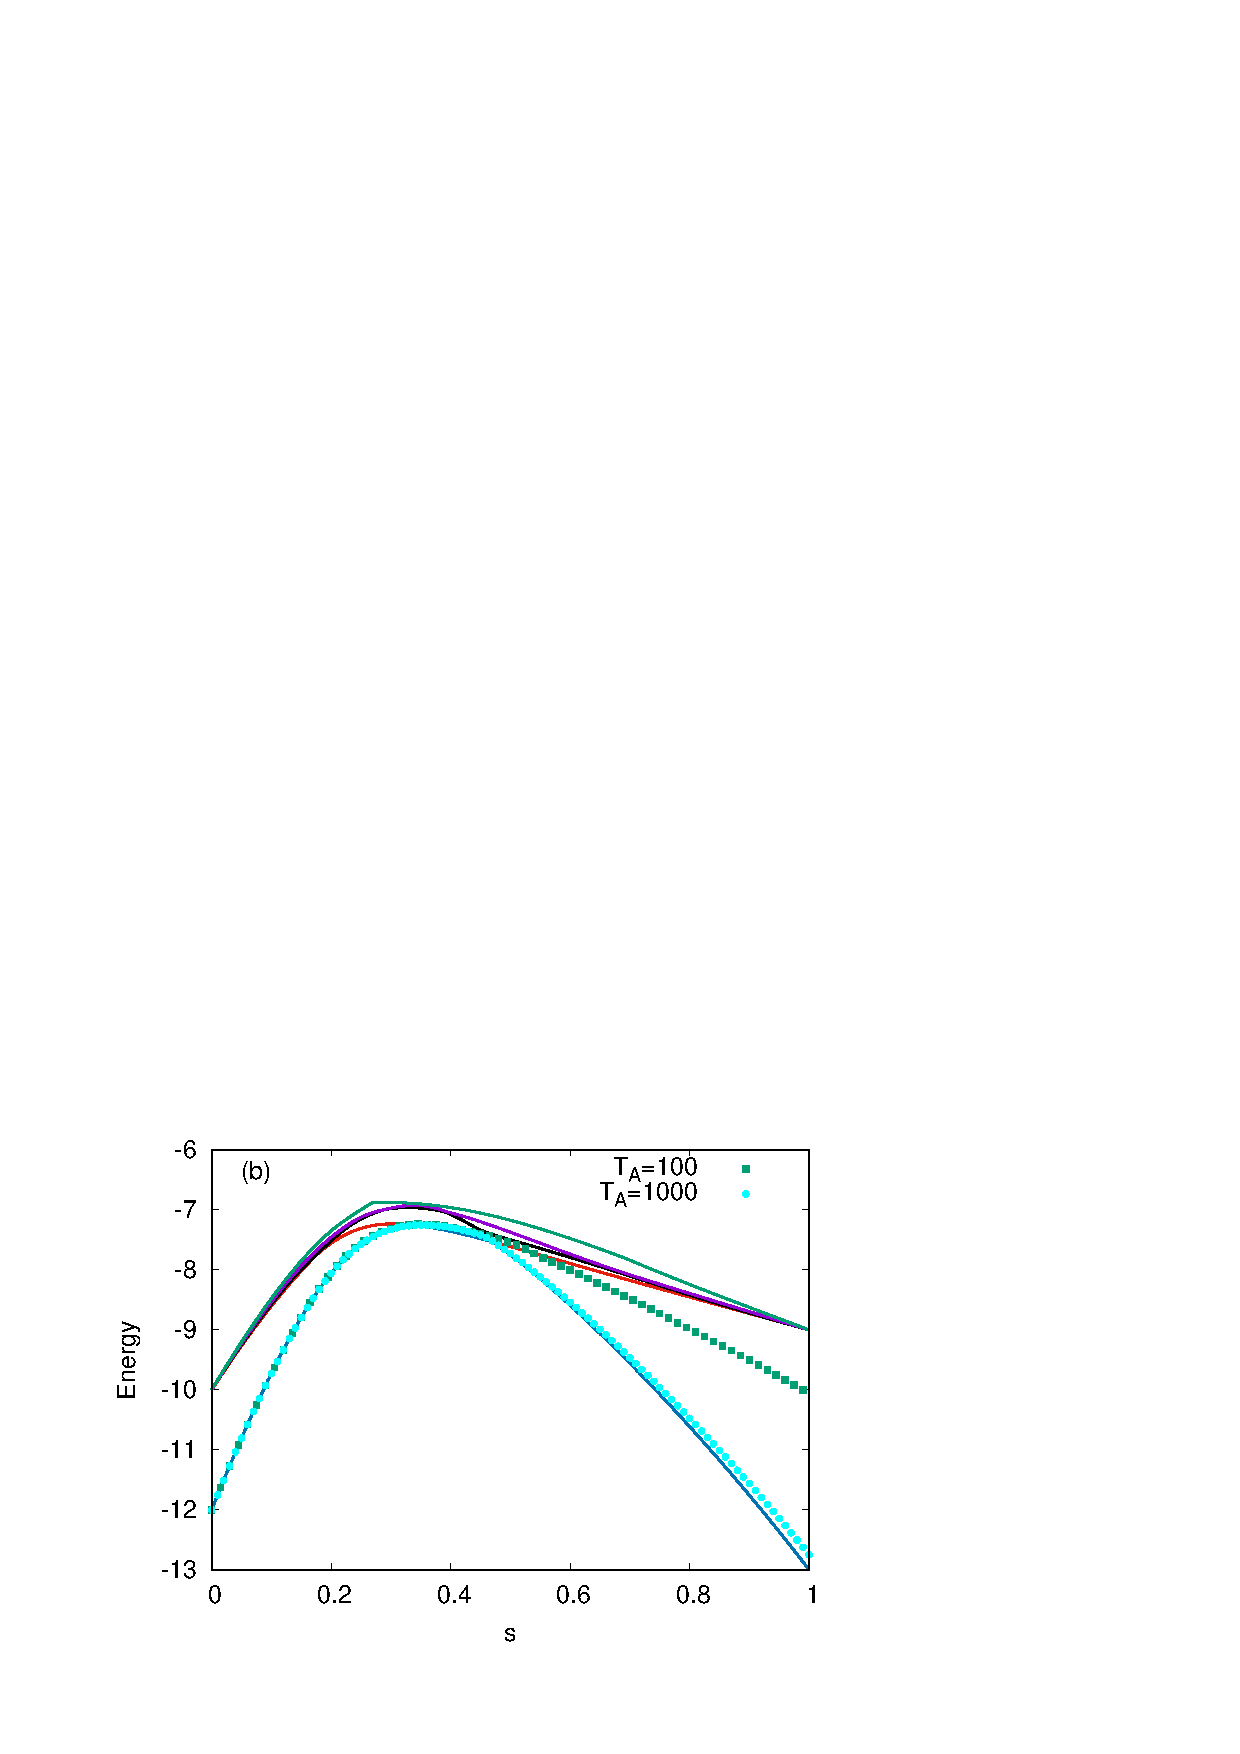
\includegraphics[scale=0.3]{441_A_g1_T100_1000.png}
\caption{A plot of the success probabilities after adding the anti-ferromagnetic trigger with g=1 ($p^A$), with the original success probabilities($p^O$) for annealing time 10, 100 and 1000.}
\label{fig:a29}
\end{figure}

In this problem, the state of the system shifts to the first excited state at the first energy anti-crossing, but transits back to the ground state at the second one. Therefore, although the minimum energy gap has become smaller, the success probability after adding the trigger increases.\\

Moreover, for cases a and e similar kind of mechanism is at play for increasing the success probability after including the trigger, despite of a decrease in the minimum energy gap. Case a was found to be the same as the second chosen problem in the first section of the chapter. It can be noted from figure (\ref{fig:a8}) that adding the trigger changes the spectrum in such a way that the ground state and the first excited state stay close to each other for a longer amount of time. When the gap between these levels starts to increase again, the system state shifts most amplitude to the ground state again.\\

It was also noted that there were additional cases in the scatter plot for the minimum energy gap ($\Delta_{min}^A$ vs $\Delta_{min}^O$) for $T_A$=100. Cases f, g and h, marked in figure (\ref{fig:a28}) were additionally studied and were found to have similar dynamics. For cases g and h the number of anti-crossing was found to have increased to 2, where both the gaps were small enough for the state to transit at $T_A$=100, hence working in favour of the success probability. 

For case f , figures (\ref{fig:a30}) and (\ref{fig:a31}) show the plots for the energy spectrum and the instantaneous energy values before and after adding the trigger.

\begin{figure}[H]
\centering 
\includegraphics[scale=0.3]{969_O_T100.png}
\caption{A plot of the success probabilities after adding the anti-ferromagnetic trigger with g=1 ($p^A$), with the original success probabilities($p^O$) for annealing time 10, 100 and 1000.}
\label{fig:a30}
\end{figure}
In this case, adding the trigger increases the number of anti-crossings to 2, while also making the energy spectrum more involved. The energy levels come close enough for the state to shift to higher or lower levels at other points than just the anti-crossings. (\textbf{Explain better.})
\begin{figure}[H]
\centering 
\includegraphics[scale=0.3]{969_A_T100_g1.png}
\caption{A plot of the success probabilities after adding the anti-ferromagnetic trigger with g=1 ($p^A$), with the original success probabilities($p^O$) for annealing time 10, 100 and 1000.}
\label{fig:a31}
\end{figure}

Again, for checking if the dynamics after adding the anti-ferromagnetic trigger with g=1 was adiabatic, the success probabilities for different problems were plotted against the corresponding minimum gaps. Figure (\ref{fig:a30}) shows the resulting plot.

\begin{figure}[H]
\centering 
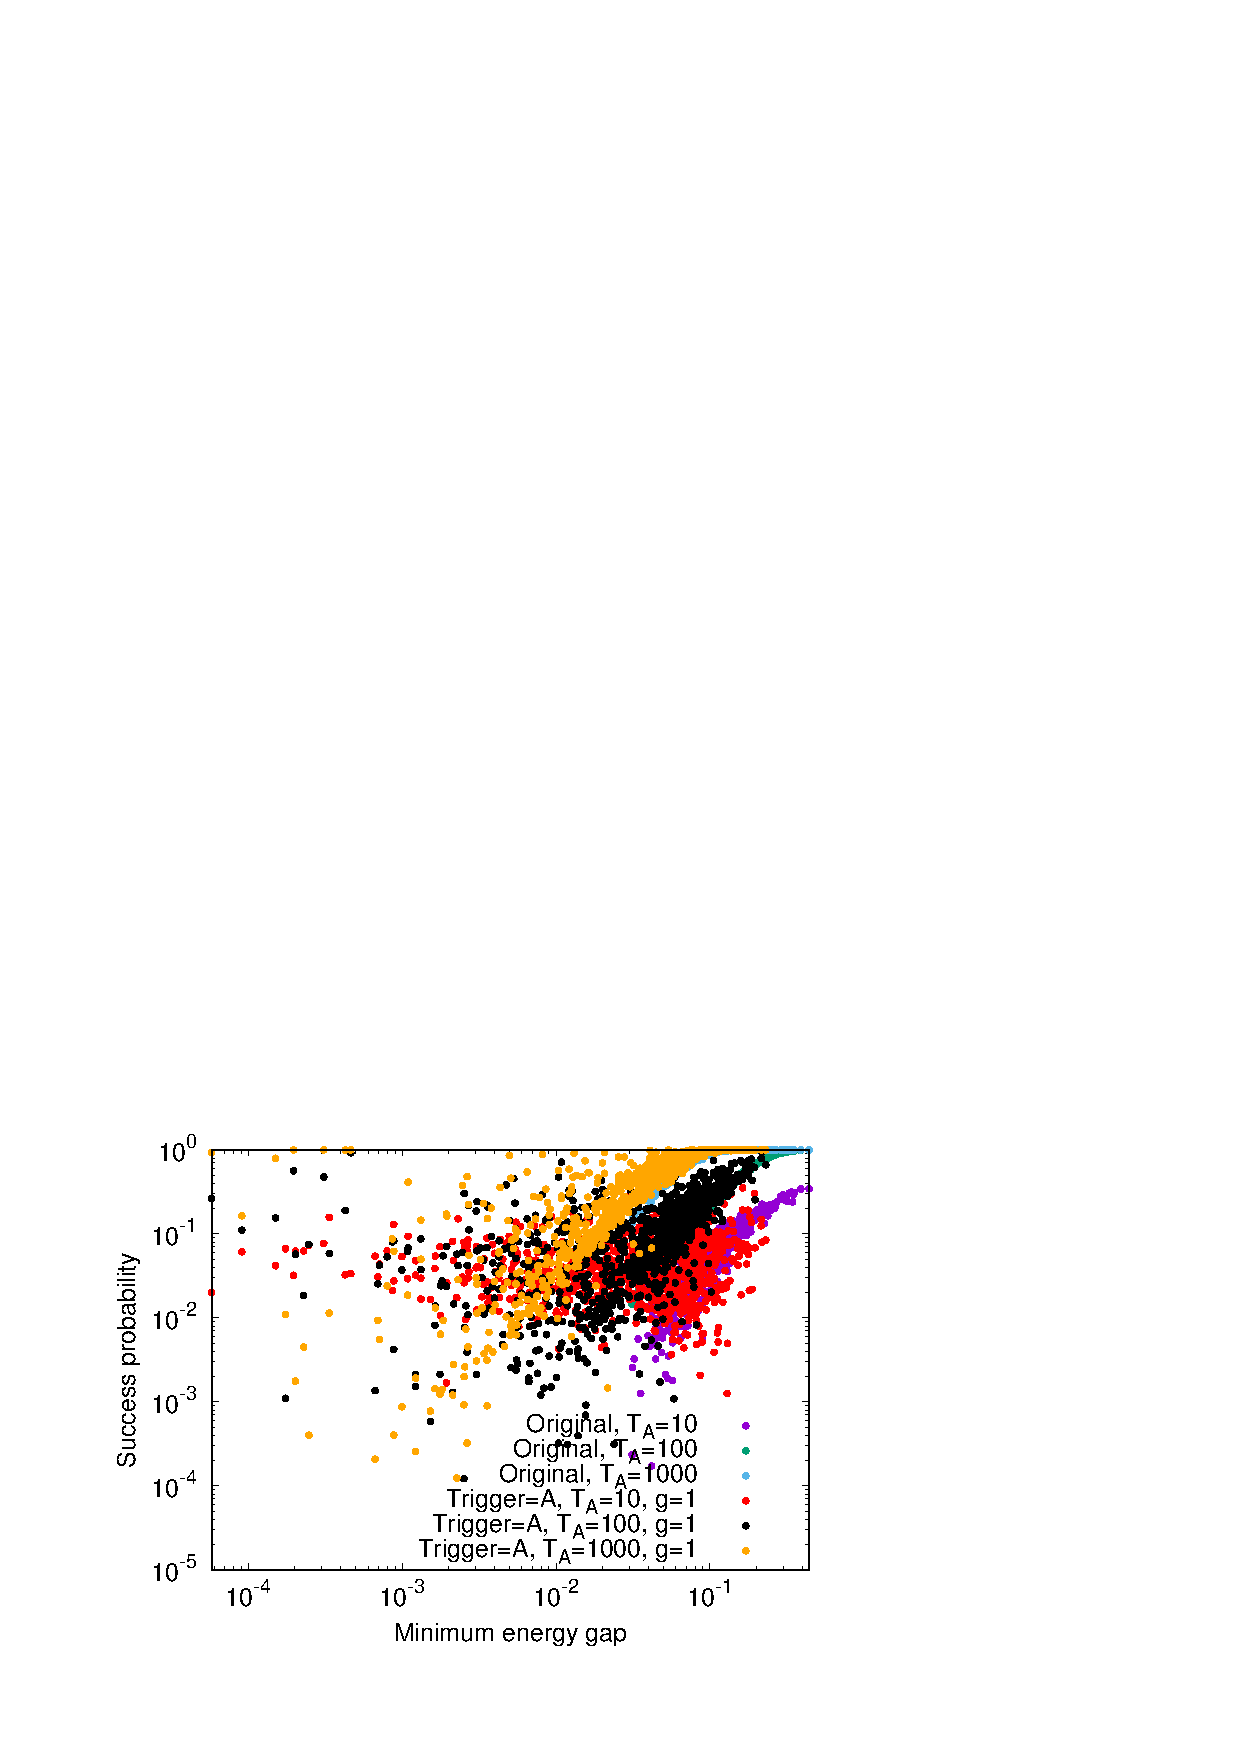
\includegraphics[scale=0.3]{SuccVsGap_OA_g1.png}
\caption{Success probability versus minimum energy plot for all the problems belonging to the set of 12-spin SAT problems, for annealing times 10, 100 an 1000, in the absence and presence of ferromagnetic trigger.}
\label{fig:a30}
\end{figure}
It can be noted that the scattering of the curves has increased substantially, although the form of the curves is defined better in this case compared to the last section (\ref{fig:a17}). (\textbf{MORE})


\section*{g=2}
Finally, in this section the effects of adding the anti-ferromagnetic with strength 2 will be discussed. 
\end{document}